% Options for packages loaded elsewhere
\PassOptionsToPackage{unicode}{hyperref}
\PassOptionsToPackage{hyphens}{url}
%
\documentclass[
]{book}
\usepackage{amsmath,amssymb}
\usepackage{lmodern}
\usepackage{iftex}
\ifPDFTeX
  \usepackage[T1]{fontenc}
  \usepackage[utf8]{inputenc}
  \usepackage{textcomp} % provide euro and other symbols
\else % if luatex or xetex
  \usepackage{unicode-math}
  \defaultfontfeatures{Scale=MatchLowercase}
  \defaultfontfeatures[\rmfamily]{Ligatures=TeX,Scale=1}
\fi
% Use upquote if available, for straight quotes in verbatim environments
\IfFileExists{upquote.sty}{\usepackage{upquote}}{}
\IfFileExists{microtype.sty}{% use microtype if available
  \usepackage[]{microtype}
  \UseMicrotypeSet[protrusion]{basicmath} % disable protrusion for tt fonts
}{}
\makeatletter
\@ifundefined{KOMAClassName}{% if non-KOMA class
  \IfFileExists{parskip.sty}{%
    \usepackage{parskip}
  }{% else
    \setlength{\parindent}{0pt}
    \setlength{\parskip}{6pt plus 2pt minus 1pt}}
}{% if KOMA class
  \KOMAoptions{parskip=half}}
\makeatother
\usepackage{xcolor}
\usepackage{longtable,booktabs,array}
\usepackage{calc} % for calculating minipage widths
% Correct order of tables after \paragraph or \subparagraph
\usepackage{etoolbox}
\makeatletter
\patchcmd\longtable{\par}{\if@noskipsec\mbox{}\fi\par}{}{}
\makeatother
% Allow footnotes in longtable head/foot
\IfFileExists{footnotehyper.sty}{\usepackage{footnotehyper}}{\usepackage{footnote}}
\makesavenoteenv{longtable}
\usepackage{graphicx}
\makeatletter
\def\maxwidth{\ifdim\Gin@nat@width>\linewidth\linewidth\else\Gin@nat@width\fi}
\def\maxheight{\ifdim\Gin@nat@height>\textheight\textheight\else\Gin@nat@height\fi}
\makeatother
% Scale images if necessary, so that they will not overflow the page
% margins by default, and it is still possible to overwrite the defaults
% using explicit options in \includegraphics[width, height, ...]{}
\setkeys{Gin}{width=\maxwidth,height=\maxheight,keepaspectratio}
% Set default figure placement to htbp
\makeatletter
\def\fps@figure{htbp}
\makeatother
\setlength{\emergencystretch}{3em} % prevent overfull lines
\providecommand{\tightlist}{%
  \setlength{\itemsep}{0pt}\setlength{\parskip}{0pt}}
\setcounter{secnumdepth}{5}
\ifLuaTeX
  \usepackage{selnolig}  % disable illegal ligatures
\fi
\IfFileExists{bookmark.sty}{\usepackage{bookmark}}{\usepackage{hyperref}}
\IfFileExists{xurl.sty}{\usepackage{xurl}}{} % add URL line breaks if available
\urlstyle{same} % disable monospaced font for URLs
\hypersetup{
  pdftitle={Glossary},
  pdfauthor={Speedgoat},
  hidelinks,
  pdfcreator={LaTeX via pandoc}}

\title{Glossary}
\author{Speedgoat}
\date{2022-11-11}

\begin{document}
\maketitle

{
\setcounter{tocdepth}{1}
\tableofcontents
}
\hypertarget{introduction}{%
\chapter{Introduction}\label{introduction}}

This manual is a support document for the IDFG PopR website, which was created to streamline the process of running population models including \protect\hyperlink{ipm}{IPM}, \protect\hyperlink{sight}{Sightability}, and \protect\hyperlink{surv}{Survival}, as well as a framework for uploading survey \protect\hyperlink{de}{data}.

At the top right of your page is a help toolbar. From left to right, the question mark brings you to the Speedgoat homepage, the little bug icon allows you to send a bug report to the speedgoat team, the lightbulb icon allows you to send the team an idea you have for a new feature, the broadcast symbol is a link to the speedgoat blog, and the lifering gives direct contact information for Josh and Paul.

Each tool has its own chapter, which includes an Overview, a Walkthrough, and a reference page for each separate section within the tools. The Overview gives a general description of what a tool is and how it works, as well as hypothetical use cases for the tool. The Walkthrough is a step-by-step guide which explains how to load data and generate analyses with each tool. The reference page gives a more detailed explanation of each page, as well as how to navigate the various menus.

Words that are {green and bold} can be found in our glossary section at the end of the book, and words that are {blue and bold} denote icon labels.

This manual was created by \href{https://www.speedgoat.io}{Speedgoat} using \href{https://bookdown.org/}{bookdown}.

Feedback and suggestions for improving the user manual are welcome at \href{mailto:wyatt.nielsen@speedgoat.io?cc=josh.nowak@speedgoat.io\&subject=PopR\%20Documentation\%20Feedback}{wyatt.nielsen@speedgoat.io}.

To get started with PopR, visit the \href{https://www.speedgoat.io/}{Speedgoat homepage} and select Idaho from the login menu.

\href{https://www.speedgoat.io}{
\includegraphics{./www/spdgt_logo.png}}

\hypertarget{ipm}{%
\chapter{IPM}\label{ipm}}

An IPM, or Integrated Population Model, combines data from many sources in its analyses for the sake of estimates that acknowledge the many factors that can influence abundance and survival. Our IPM uses data from survival and sightability models, as well as harvest data from the IDFG database to calculate rates like survival and sex ratios for an entire {DAU}, extrapolated to the entire unit and better informed by all the different metrics that are considered in the process of fitting the model.

\hypertarget{ipm-model}{%
\section{Walkthrough}\label{ipm-model}}

Using the IPM tool can be split into two major processes: preparing data and looking at data.

\hypertarget{ipm-load}{%
\subsection{Preparing Data}\label{ipm-load}}

Click on the Setup tab, the first dropdown under the IPM tool menu.

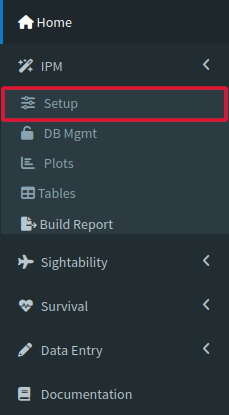
\includegraphics{./www/ipm_walk1.png}

On the top left of the page should be a window labeled Overview, and this is where you determine the data that you run through the IPM. Select the database you want to retrieve the data from, then make sure you choose your Species, {DAU}, Unit, and Weather before you click {Fetch Harvest Data} on the bottom right of the Overview window to retrieve the specific data you requested.

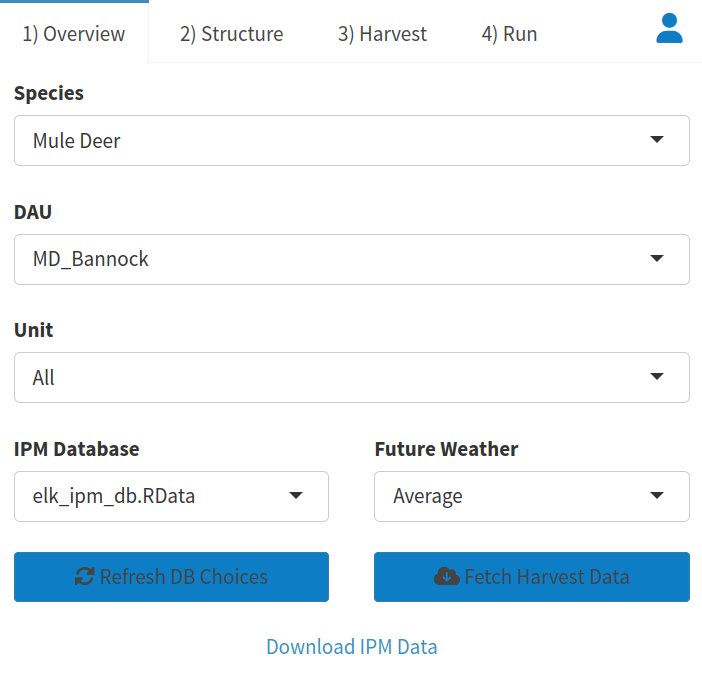
\includegraphics{./www/ipm_walk2.png}

Once the data is loaded, you should get a popup dialog letting you know that the process was successful. It will also prompt you to proceed to the ``Structure'' tab (At the top left of the page next to the Overview tab), which is where we will continue our data preparation.

The Structure tab allows you to select whether your survival and reproduction will have a constant or time varying data variance. The defaults were chosen to be well-suited to a variety of situations, so most of the time clicking {``Default Structure''} will be all you need to do here. Often the inputs that appear when the tool is opened are actually not the same as those that are selected when you press {``Default Structure''}, so make sure you click that before you move on to Harvest if those are the inputs you are planning to use.

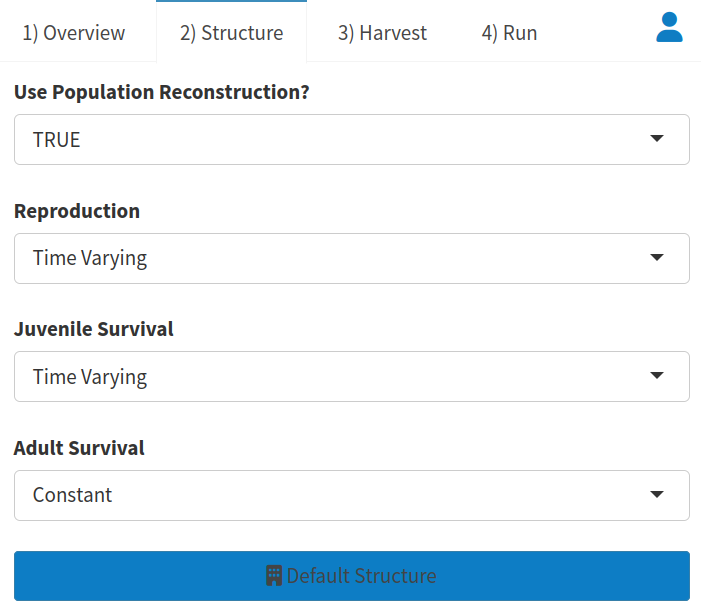
\includegraphics{./www/ipm_walk4.png}

After you select your Structure, you can move on to the Harvest Tab. Decide your effort variable and the years that you will be conducting your analysis, then look at the given information for the years that will be forecast. You can change the Harvest by double clicking the numbers and typing in new entries.

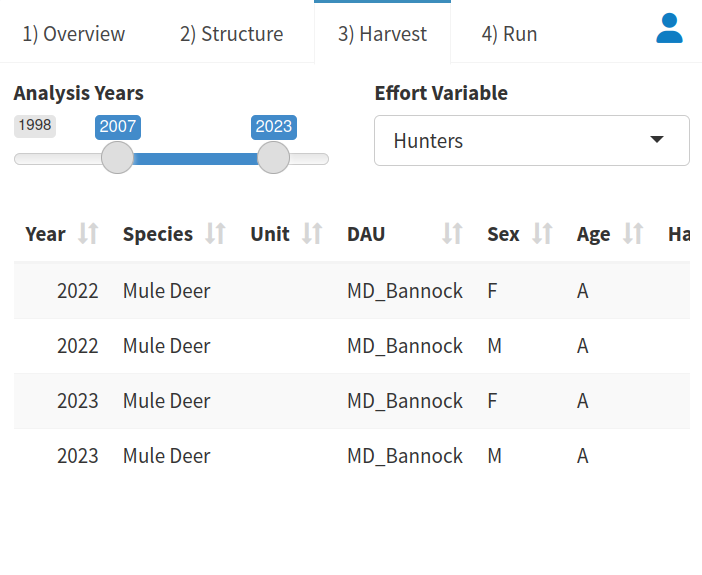
\includegraphics{./www/ipm_walk5.png}

Our next step is the Run tab, which again already has a decent set of default values loaded. Adjust your Burnin Length, MCMC iterations, and Thinning Length. Decide whether you would like to automate convergence (This may increase the time it takes to run the model).

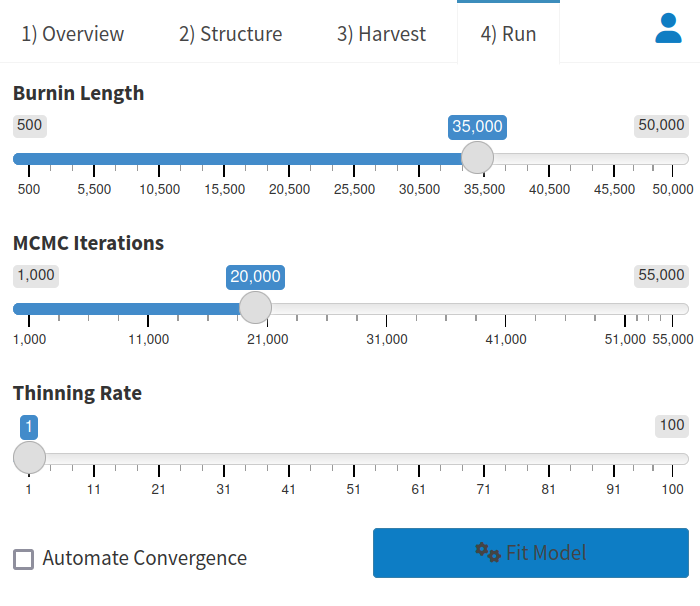
\includegraphics{./www/ipm_walk6.png}

Once you are satisfied with all of the inputs outlined above, click {Fit Model} to begin analysis. This should take some time, but you will get a dialog box letting you know when the process is complete

\hypertarget{ipm-look}{%
\subsection{Looking at Data}\label{ipm-look}}

(NOTE: This section will only work if you completed the steps above to prepare your data and fit your model beforehand.)

To look at the data you prepared, wait until the model that you initiated in the setup tab has finished running, then go ahead and click the Plots tab on the IPM dropdown menu to check the results. Hovering your mouse over a point on a plot will give you the parameter, year, age, sex, control limits, and mean associated with the dataset that created the data point.

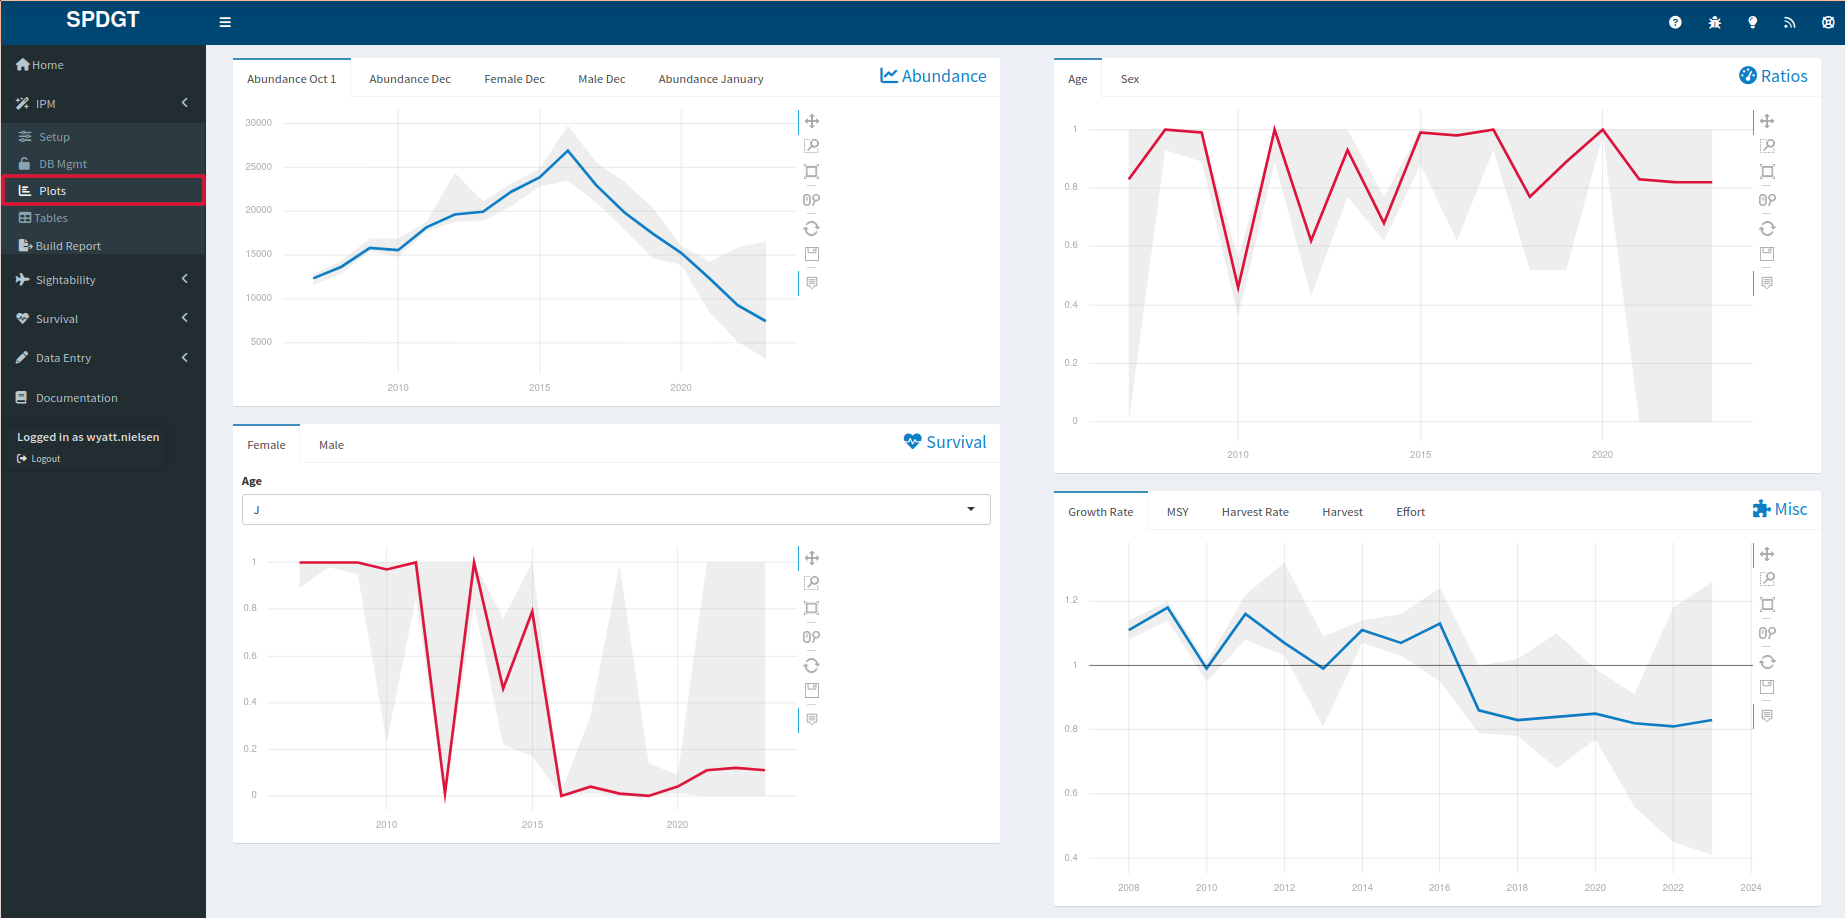
\includegraphics{./www/ipm_walk7.png}

You can also check the model output by clicking the Tables tab right below the Plots one on the IPM dropdown. Rhat values greater than 1.1 are highlighted in red, which means the model may not have converged and should be run again after modifying the settings on the Run tab in the Setup tool. The first ten entries that appear when you open the table tab are not the only outputs of the model. You will notice that you may navigate the pages with the list to the bottom right, or you may increase the number of entries visible at the top left of the page, using the {Show (10) Entries} dropdown.

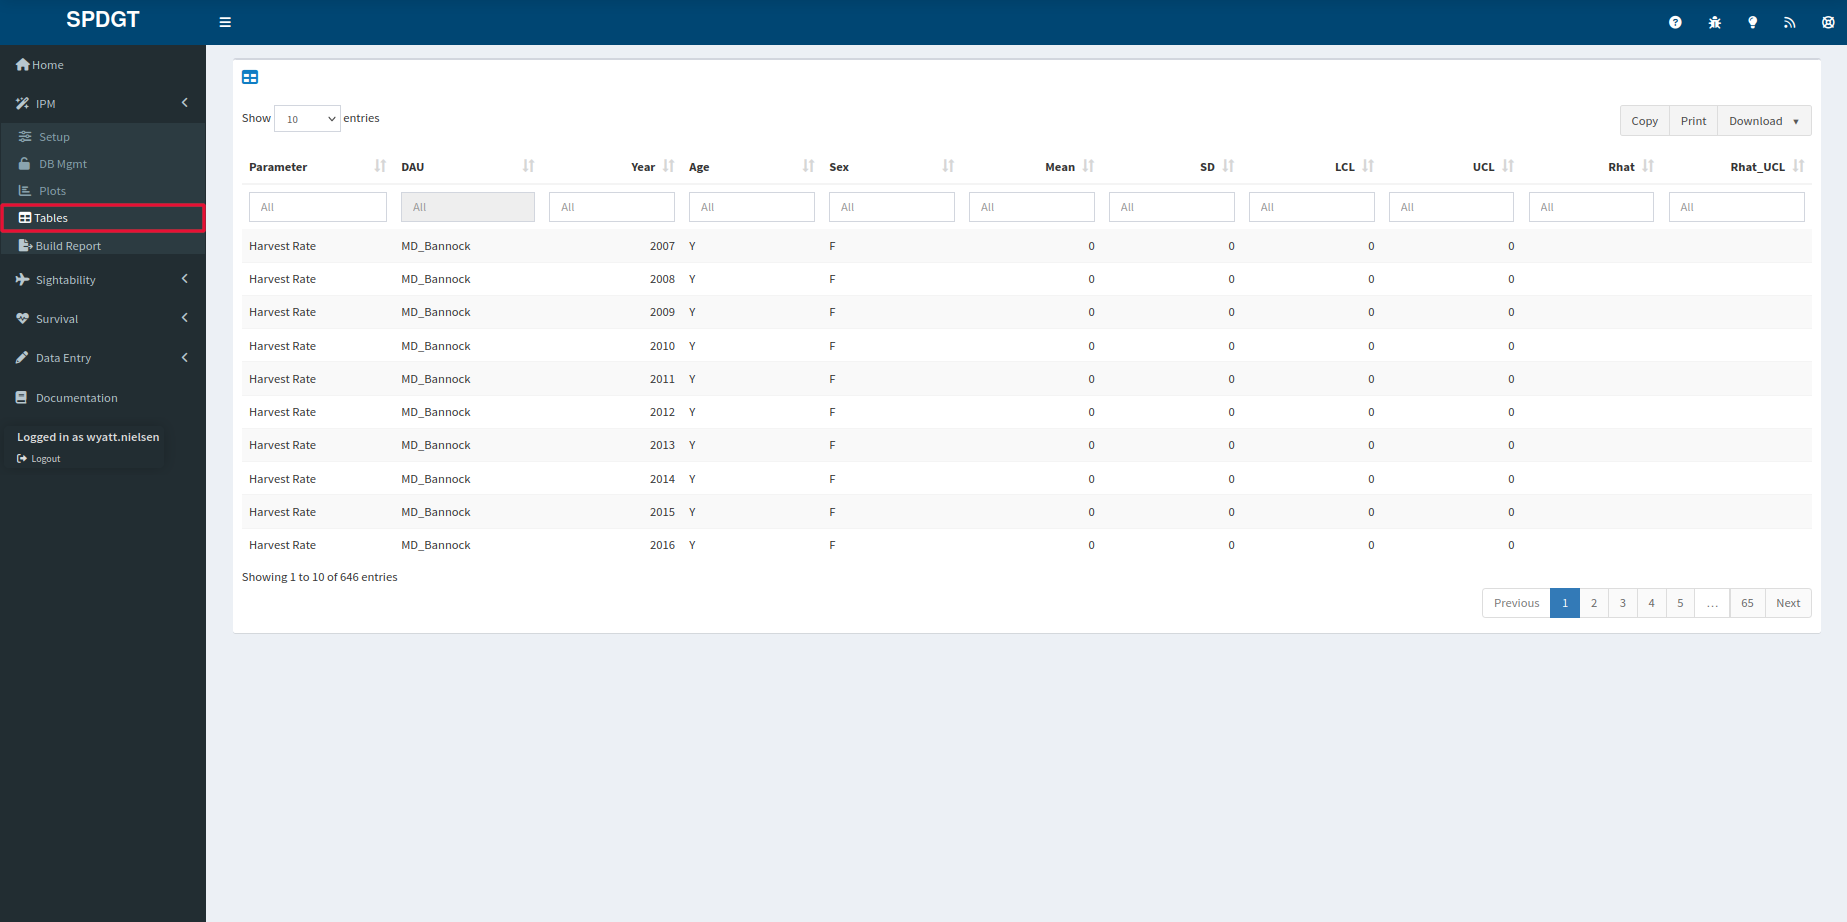
\includegraphics{./www/ipm_walk8.png}

As a final step to get more diagnostic information, use the Build Report tool.

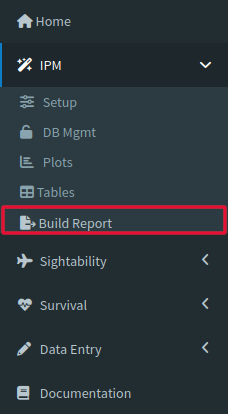
\includegraphics{./www/ipm_walk10.png}

Simply click on the tool and then click the download prompt on the popup window. The resulting document contains interactive plots as well as model specifications and fit.

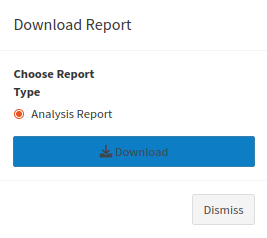
\includegraphics{./www/ipm_walk9.png}

\hypertarget{ipm-ref}{%
\section{Reference}\label{ipm-ref}}

\hypertarget{ipm-setup}{%
\subsection{Setup}\label{ipm-setup}}

The main purpose of the Setup tab is to load and preview data that will be used for later analysis, and we will spend more time describing each element in detail. The window on the top left of the page has several tabs related to data preparation labeled Overview, Structure, Harvest, and Run.

The Overview tab helps you find the data you will be loading for your IPM. Make sure that you are pulling from the correct database! Also, the Future Weather dropdown allows you to consider weather in your IPM analysis. Average assumes mean observed weather conditions, Good assumes upper 95\% quantile of observed weather, and Bad assumes lower 5\% quantile of observed weather. You may also choose not to include weather in your analysis. All of these values were developed from the dissertation of Mark Hurley.

The Structure tab gives our model some information about assumptions. Population reconstruction is the process of estimating past abundance using a combination of known harvest data and estimated natural mortality rates. If you know when an animal died AND how old it was when it died, then you also know when it was alive. Using this ``back-tracking'' can create an abundance estimate for past years even if one was not carried out.

The Harvest tab gives our model some important context on harvest metrics. The slider at the top tells our model which years are being analyzed. The effort variable allows us to choose whether effort is determined by the number of days in the field or the number of hunters themselves. It also gives more context to our harvest numbers and helps us tease apart the relationship that hunter effectiveness and raw number of hunters had on the harvest that year. You may also give hypothetical harvest numbers for our model to consider so you may estimate the effects of management decisions on rates like survival and abundance.

The Run tab gives direction to our actual modeling process. The given settings control how we deal with the many thousands of times the model must run to calibrate itself. Burnin Length helps us focus our model. When the MCMC model begins running, it checks possible outputs of the model and begins sampling them to determine the probability that they will represent our data. The model uses past sampled points to try and get an idea of where the highest probabilities are, but when the model first begins running it does not have the luxury of these reference points. This sets up the model's first few samples to be more randomly chosen than any part of the process, meaning that the beginning samples are less likely to be on high probability outputs. Burnin Length helps us get around this by deleting the first runs of the MCMC model after it's done running. MCMC iterations is simply a measure of how many different times the model will test the probability of different model outputs. More sampling allows the model to consider more options and therefore can increase the chance that the model will find the outputs with the highest likelihoods, but it also may not be necessary and will make the tool take longer to run. Thinning rate helps us save memory by deleting entries from the model's stored runs. We can think of this as a sort of browser history for the model, showing us how it got its answer. In this case there are literally tens of thousands of steps, so deleting a small (or large) proportion of that history and using what is left still gives us an idea of the model's actions without taking up nearly as much memory. The slider is the percentage of model iterations that will be deleted once the modeling process is complete.

The window on the top right of the page is for previewing data after it is loaded but before the model is run. Hovering your cursor over data points will give you all relevant data. You can change your view of the data using the pan and two zoom features on the side of each graph. Click the reset button to return to the original view. The table at the bottom of the page gives another way to preview the data you loaded in the Overview tab. You can organize your data by any of the column headers, and note that you can navigate and view more of your data with the previous and next buttons at the bottom of the page.

\hypertarget{ipm-dbmgmt}{%
\subsection{Database Management}\label{ipm-dbmgmt}}

The DB Mgmt tab creates, deletes and edits databases.The tools may be minimized, but to open them for use just click on the plus sign on the right side of the box containing the tool. Press it again to minimize it. Note that because databases are shared between users, edits here will change databases for EVERYONE. Data losses and changes will be permanent if you do not back up your data. You can also use the Create tab to make a new database.

You can enter your information manually using the blank table at the bottom of the tool window, but you may also paste data from a spreadsheet app like Excel. You can also start off with data from any existing database, which you can select under the Historic Data box. Make sure to give your new database a name, and then click the create database button to add a database to the Speedgoat server! You can also use the download tool to get the data you have loaded into our servers as a .csv.

The Delete DB tool will delete the database you select from the server. Deleting it here will delete it for everyone, so make sure that your data is backed up and that nobody is still working on a database before you delete it.

The Edit tool allows you to add and delete rows of data from the database selected in the menu at the top of the tool. None of the edits you make will be applied until the Save Changes button is clicked, but once that button is clicked changes will be applied for everyone that uses that database.

\hypertarget{ipm-plot}{%
\subsection{Plots}\label{ipm-plot}}

The plots page has graphs that are created by running your selected data through an IPM. Use the zoom and pan tools to change your view of the graph, and use the reset button to return to your original view.

\hypertarget{ipm-table}{%
\subsection{Tables}\label{ipm-table}}

On the Tables page you can download and edit the data you are using for analysis. You can download your data here as well, but note that you will only download the data being displayed to you. By default, the table only shows the first ten entries of your dataset, so if you would like to download your data here make sure you change the dropdown at the top of the window from Show 10 entries to Show All entries.

\hypertarget{ipm-report}{%
\subsection{Build Report}\label{ipm-report}}

The Build Report tool gives a summary of the analysis conducted, while keeping relevant information like model settings for future comparisons.

\hypertarget{sight}{%
\chapter{Sightability}\label{sight}}

Sightability models estimate abundance in a unit by combining the number of animals that we have seen in aerial surveys with an estimated number of animals that we have NOT seen using detection probability models. These detection models consider ground vegetation, the animal's activity, snow cover, and the size of the group of animals to determine the likelihood that an animal is seen with the interference of these variables.

Stratum are used to organize habitat subunits by how well they would work as habitat for the animal being surveyed. The ``high'' strata group represents subunits that contain the best habitat, ``low'' is the group that has the worst habitats, and ``medium'' falls in between. Subunits are determined by previous observations from biologists and snow cover.

\hypertarget{sight-walk}{%
\section{Walkthrough}\label{sight-walk}}

Using the Sightability tool can be split into two major processes: preparing data and looking at data.

\hypertarget{sight-prep}{%
\subsection{Preparing Data}\label{sight-prep}}

To prepare the data, navigate to the Setup tab under the Sightability dropdown.

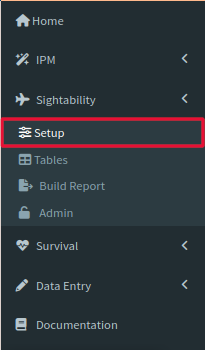
\includegraphics{./www/sight_walk1.png}

Within the setup section, the User Inputs window decides which survey data you will load. Select your species, {DAU}, Survey Type, Year, Analysis Focus, and Aircraft/Model. The data preview on the right side of the page will update as you adjust your settings. Check it as you make your choices in the User Inputs window, but you do not have to modify it any further.

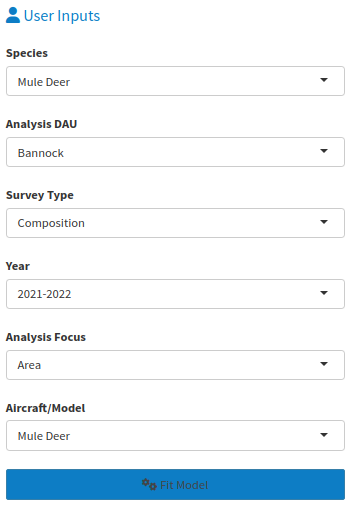
\includegraphics{./www/sight_walk2.png}

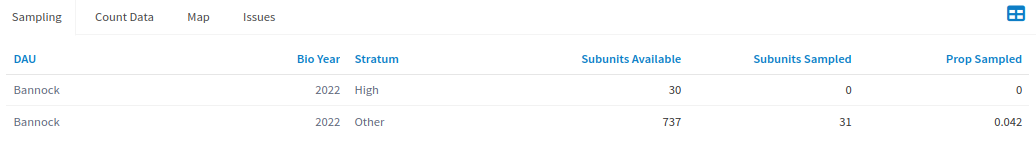
\includegraphics{./www/sight_walk3.png}

Once you are satisfied with your choices in the User Input window, go ahead and click {Fit Model}. You will get a dialog box letting you know when the tool ran successfully.

\hypertarget{sight-look}{%
\subsection{Looking at Data}\label{sight-look}}

Now that your data has been prepared you can go to the Tables tab, which is where you can view the output of your model.

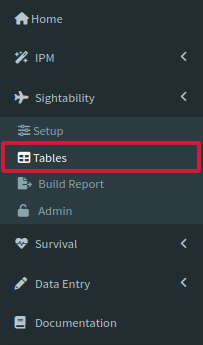
\includegraphics{./www/sight_walk4.png}

Navigate with the tabs along the top of the screen to check your estimates, survey design, detection, and covariates. You can also download your detection and estimation results as .csv files with {Download} at the bottom of the table.

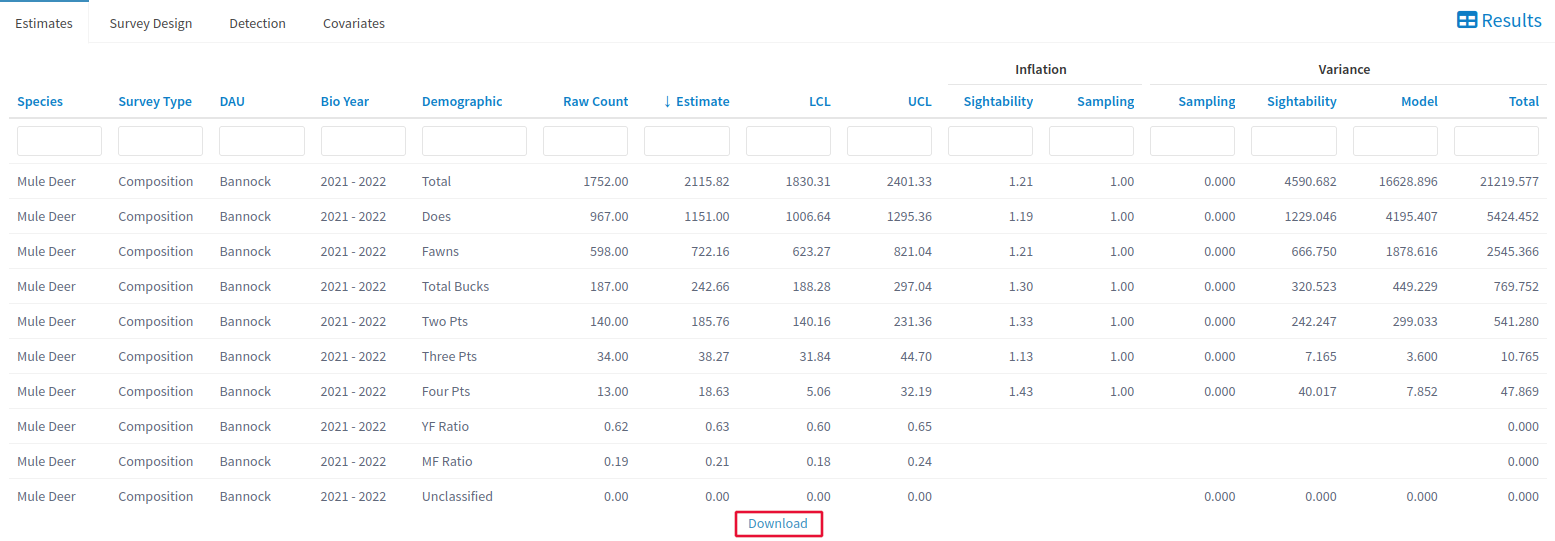
\includegraphics{./www/sight_walk5.png}

To get a more detailed report of your model that includes the information in the Tables tab while keeping track of things like model settings, click the Build Report tab under Sightability. A prompt will appear asking you to download the report as an html file.

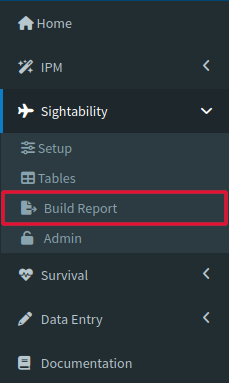
\includegraphics{./www/sight_walk7.png}

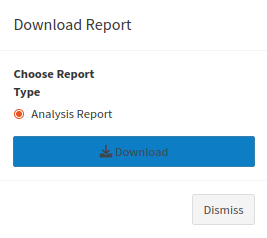
\includegraphics{./www/ipm_walk9.png}

If you would like to upload the results of your model to an IPM database, you can click on the Admin tab.

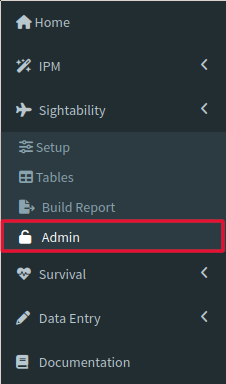
\includegraphics{./www/sight_walk6.png}

EDITS HERE WILL EDIT DATABASES FOR EVERYONE. You can select the database that you want to upload your data to, as well as review the information that you will be uploading. Press {Update DB} to add your selected results to a shared database.

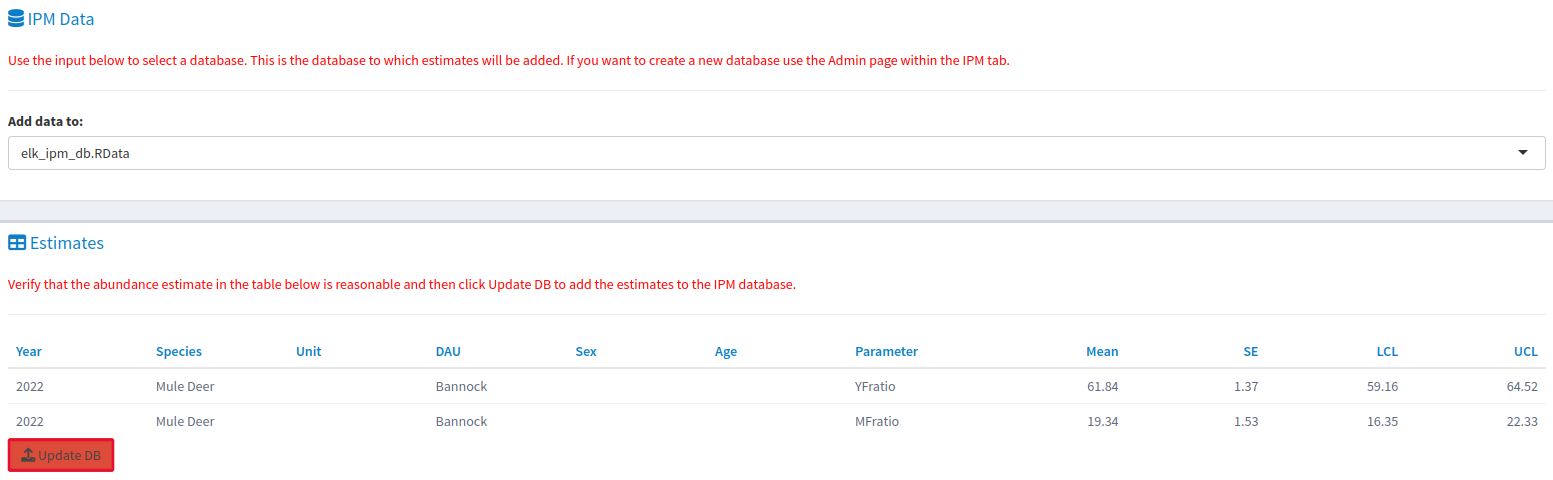
\includegraphics{./www/sight_walk8.png}

\hypertarget{sight-ref}{%
\section{Reference}\label{sight-ref}}

\hypertarget{sight-setup}{%
\subsection{Setup}\label{sight-setup}}

The setup tab is used to select which {DAU} will be run through our model.

The User Inputs tab on the left side of the screen allows you to specify which data we will be analyzing. Surveys will only appear if they are a perfect match to all of the dropdown menus, so make sure to double check that you did not accidentally leave one of them as default if the survey you are looking for refuses to appear in the preview window. The species dropdown allows to to choose whether you are selecting elk surveys or mule deer surveys.

The Analysis DAU dropdown selects which region of Idaho we will be analyzing. All DAUs in Idaho are included as options for a survey, but this does not necessarily mean that surveys from every DAU have been uploaded to the speedgoat database. If nothing appears in the preview window on the right side of the screen when you select a DAU, then it means there is no data available. The Survey Type dropdown includes both {composition} and {sightability-abundance} surveys. The year tab refers to which Biological year the survey was carried out on. Years are referred to as ``2016-2017'' rather than just one year because surveys are generally carried out between late fall and early spring, which straddles new year's. This makes more sense to keep related surveys together because two surveys may be flown only three weeks apart but still be lumped into separate years. If you are having trouble finding your survey, make sure you select the right time range, since a survey flown in 2016 could be in the 2015-2016 group OR the 2016-2017 group. The Analysis Focus dropdown determines what scale the analysis will be carried out within the DAU you selected. Aircraft/Model refers to which specific model type you will be running, since Elk sightability models take into account the specific make of the plane used for the survey.

\hypertarget{sight-table}{%
\subsection{Tables}\label{sight-table}}

The Tables tab allows you to look at the output of your model run from Setup. The Estimates tab displays model outputs based on your survey information, including abundance estimates for all age and sex demographics as well as Male:Female and Young:Female ratio. You can search each row with the blank box at the top. The Survey Design tab gives model settings for reference, as well as the proportion of subunits sampled and the abundance estimate for the area that you selected in Setup. The Detection tab gives raw survey info that the model used for its estimates. Notice that the page of data being displayed is only one of many pages which you can navigate with the page list on the bottom right of the window. Use the download button at the bottom of the Estimates and Detections tabs to download those results as a .csv. The covariates tab gives you a glimpse into how our models work by showing the covariate options, their {model values}, and their {beta}. This is not a table of outputs, but rather an insight as to how our model interprets the data you put into it. For example, while it would be tempting to spend precious time on a survey flight determining a specific snowcover percentage, a look at the covariates tab will tell you that snowcover is actually a categorical variable. Specifically, snowcover has three categories (1\%-20\%, 21\%-79\%, 80\%-100\%), which means that finding an exact percentage is a waste of time, since all values within the discrete categories will be treated the same. The reason you cannot see the 80-100\% category on the covariates page is because of how our model interprets snowfall. Instead of three separate categories, all categories are in terms of the 80\%-100\% one. Our model does not think of the 1\%-20\% and 21-79\% categories as independent, but as (80\%-100\% category) - (some value). 80\%-100\% is the default category, and default values are not displayed in the table.

\hypertarget{sight-report}{%
\subsection{Build Report}\label{sight-report}}

The Build Report tab prints your model outputs from the tables tab and saves model settings. Clicking the Build Report button will open a popup menu, click the download button to download the file to your machine as an HTML file.

\hypertarget{sight-admin}{%
\subsection{Admin}\label{sight-admin}}

The Admin tab is used to upload the results of your model to your database of choice. The bottom window can be used to preview the data that you plan to upload,so make sure you are comfortable with your results before you upload them to the public database. Data you upload will be incorporated into everyone else's model runs, so be careful.

\hypertarget{surv}{%
\chapter{Survival}\label{surv}}

Survival is something often calculated in a classroom setting, but the practicalities of calculating it in the real world can make things very tricky. Small sample sizes that can be found in collar studies can present a few problems, even if everything goes to plan. For example, if a collar study is composed of 4 animals, 3 of them may die (maybe it was deer opener). However, our Kaplan Meier model is telling us that 75\% of our deer are dead! Is survival for that year really 0.25? Unless you know of some catastrophe this is very unlikely. Our five deer study poses another problem, which is that the hypothetical 0.2 we produced earlier is one of only 5 possible survival rates that can come from this population!(0, 0.25, 0.5 ,0.75, 1) If true survival is 0.66, then we have a problem because there is no possible way to get that output from our model. All of this is assuming that things go to plan, things like:\\

All deer were collared at the same time\\
All dead deer were found with their collar\\
All collars worked for the duration of the study\\

Things often do not go to plan, and so more complicated models need to be created to account for for the reality of survival studies. Our model considers mortality and survival data from the entire state of Idaho as well as information from your particular DAU of interest. If there is sufficient data for your target DAU the model will use that information, but in the case that there isn't enough, the model can dip into a state-wide database that includes all capture and mortality data for the month in order to fill in gaps. Keep this in mind when your data is scarce, as the less data you have the closer your estimate will come to the state average.

\hypertarget{surv-walk}{%
\section{Walkthrough}\label{surv-walk}}

Using the Survival tool can be split into three major processes: preparing data, looking at data, and uploading data.

\hypertarget{surv-prep}{%
\subsection{Preparing Data}\label{surv-prep}}

The first step is to obtain your data. Click Setup under the Survival dropdown.

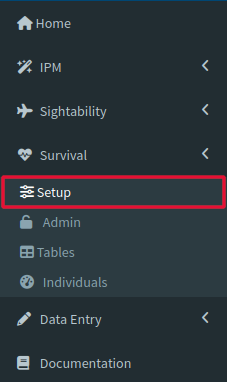
\includegraphics{./www/surv_walk1.png}

You will notice a window at the top left of the page labeled Overview, and this is where you will decide the species and DAU that we will be analyzing. Once you have made your selections, click {Download Data} at the bottom of the window.

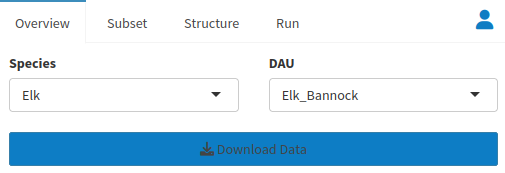
\includegraphics{./www/surv_walk2.png}

Now that your data is loaded, feel free to look it over using the windows to the right of and below the Overview window.

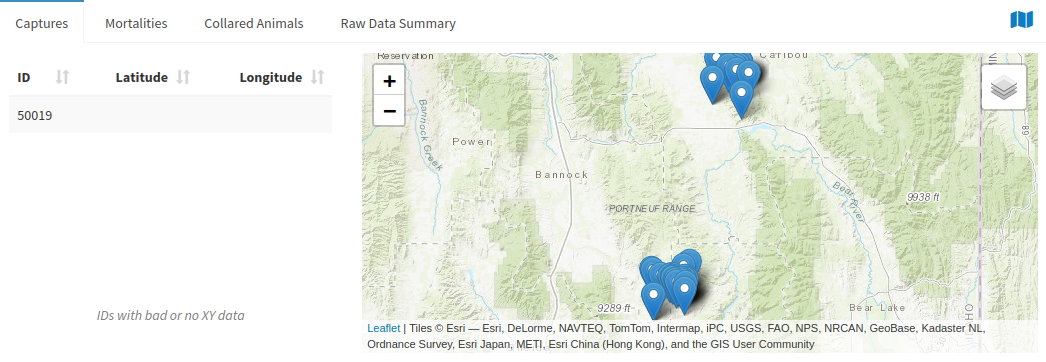
\includegraphics{./www/surv_walk3.png}

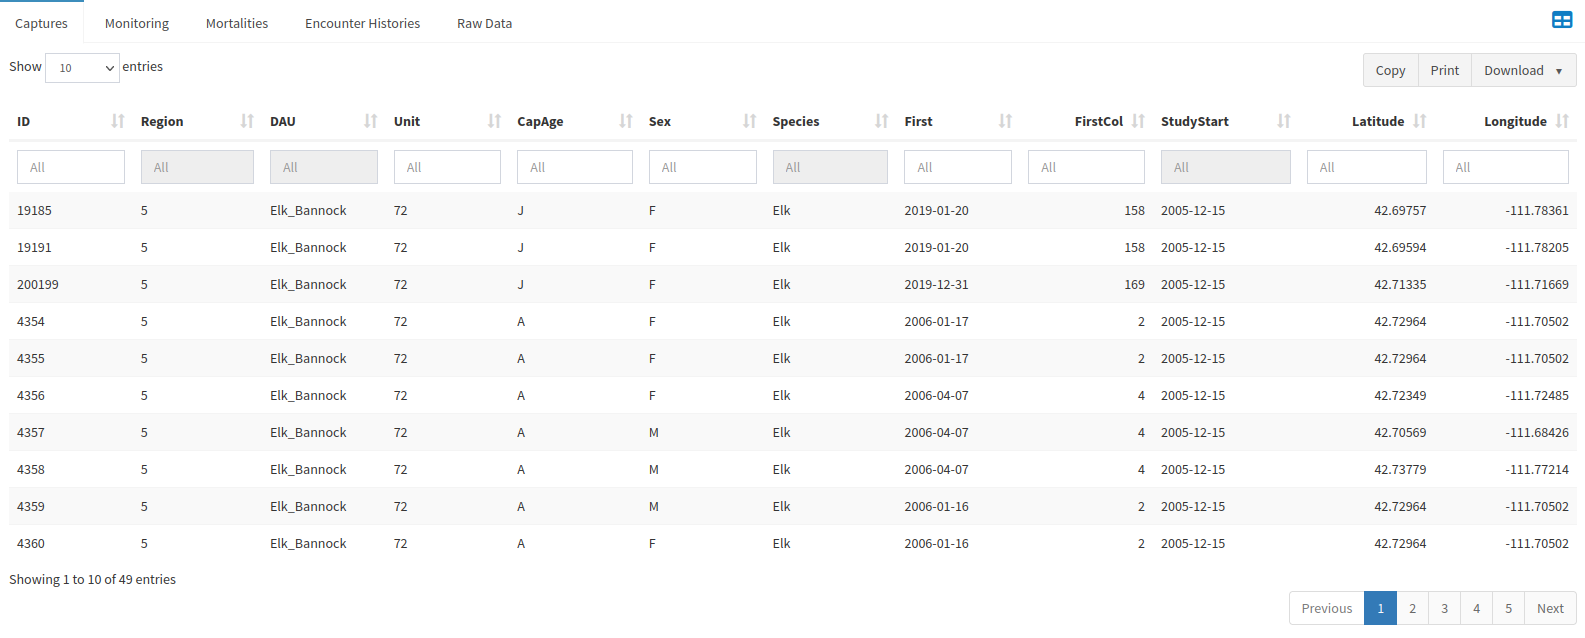
\includegraphics{./www/surv_walk4.png}

Once you have looked over your data, we can move on to the next step by navigating to the Subset tab next to the Overview one. Select the sex and age of the animals you will be analyzing, as well as the years your analysis will take place.

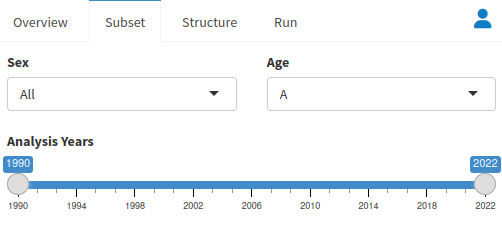
\includegraphics{./www/surv_walk5.png}

We will next move on to the Structure window, where we will determine our model type, as well as our variances for sex, time, and space. We can also choose to censor harvest mortalities.

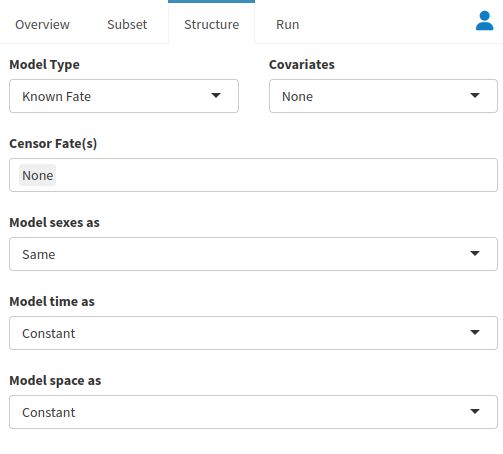
\includegraphics{./www/surv_walk6.png}

Once you have made your choices, you can move on to the Run tab. Under the run tab, decide your Thinning Rate, Burnin Length, and MCMC Iterations, then decide whether or not you would like to automate convergence. We have provided a set of defaults that are well suited for a variety of situations, but feel free to modify the values to better fit your situation.

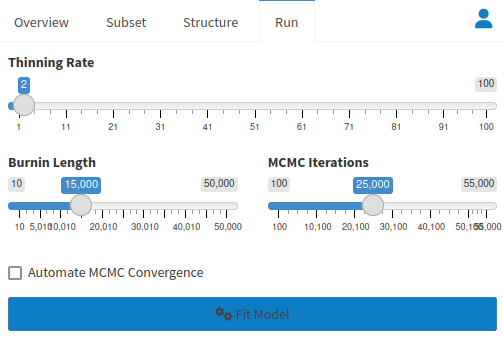
\includegraphics{./www/surv_walk7.png}

When you are done, click {Fit Model} to run the analysis. You will get a dialog box when the process is done.

\hypertarget{surv-look}{%
\subsection{Looking at Data}\label{surv-look}}

Once your model is finished running, you can view the results in the Tables tab.

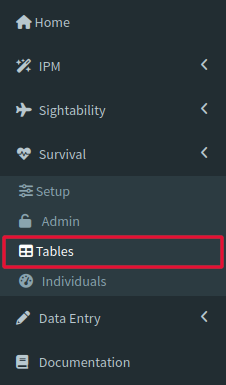
\includegraphics{./www/surv_walk8.png}

Note that the first ten entries that appear when you open this page are only a small fraction of the total. Use the page list on the bottom right to see more pages of data or use {Show (10) Entries} on the top left to make more entries appear on each page.

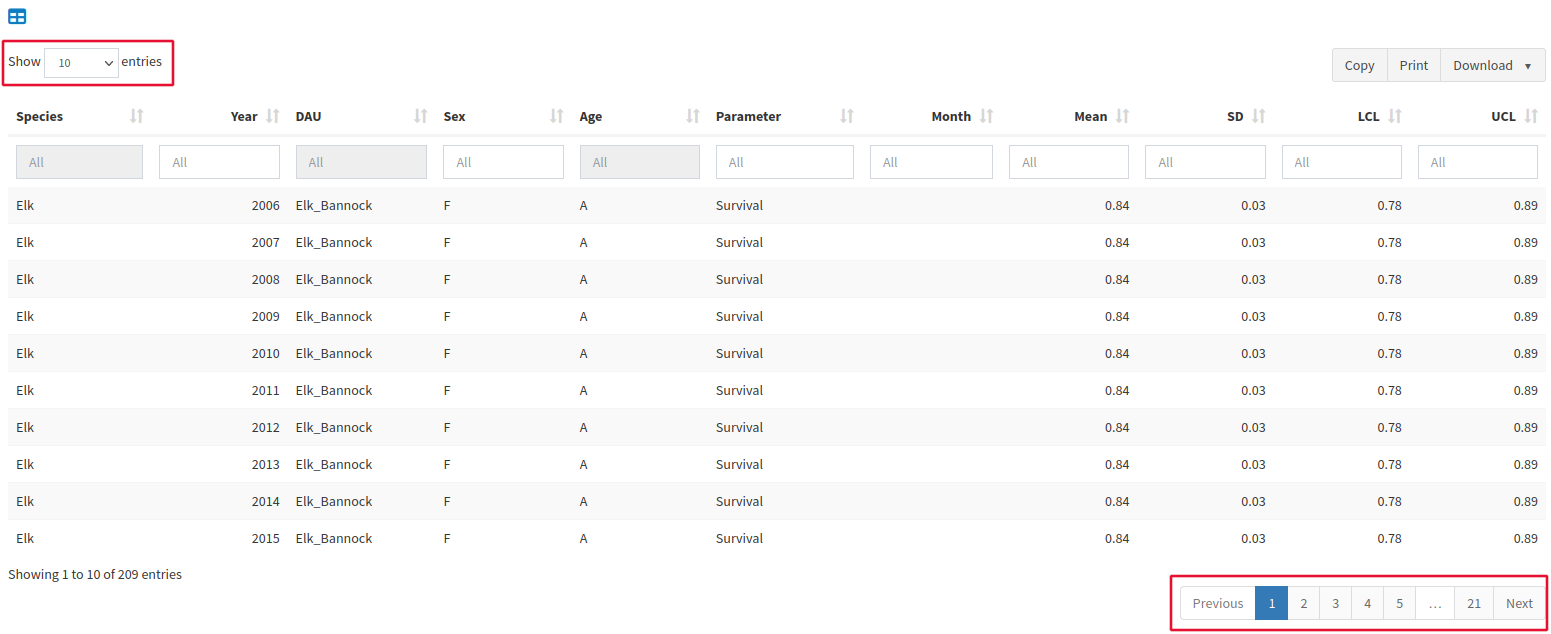
\includegraphics{./www/surv_walk9.png}

\hypertarget{surv-upload}{%
\subsection{Uploading Data}\label{surv-upload}}

If you're feeling confident about your results, you can add them to an IPM database using the Admin tab, but understand that EDITS YOU MAKE HERE WILL EDIT THE DATABASE FOR EVERYONE, which is why we ask that you're confident about your results before you add them.

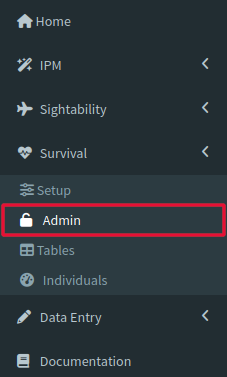
\includegraphics{./www/surv_walk10.png}

The IPM Data window allows you to select which database will receive your data, and the Estimates tab allows you to review the data that you will be adding to the database. {Update DB} will upload your data when you are ready.

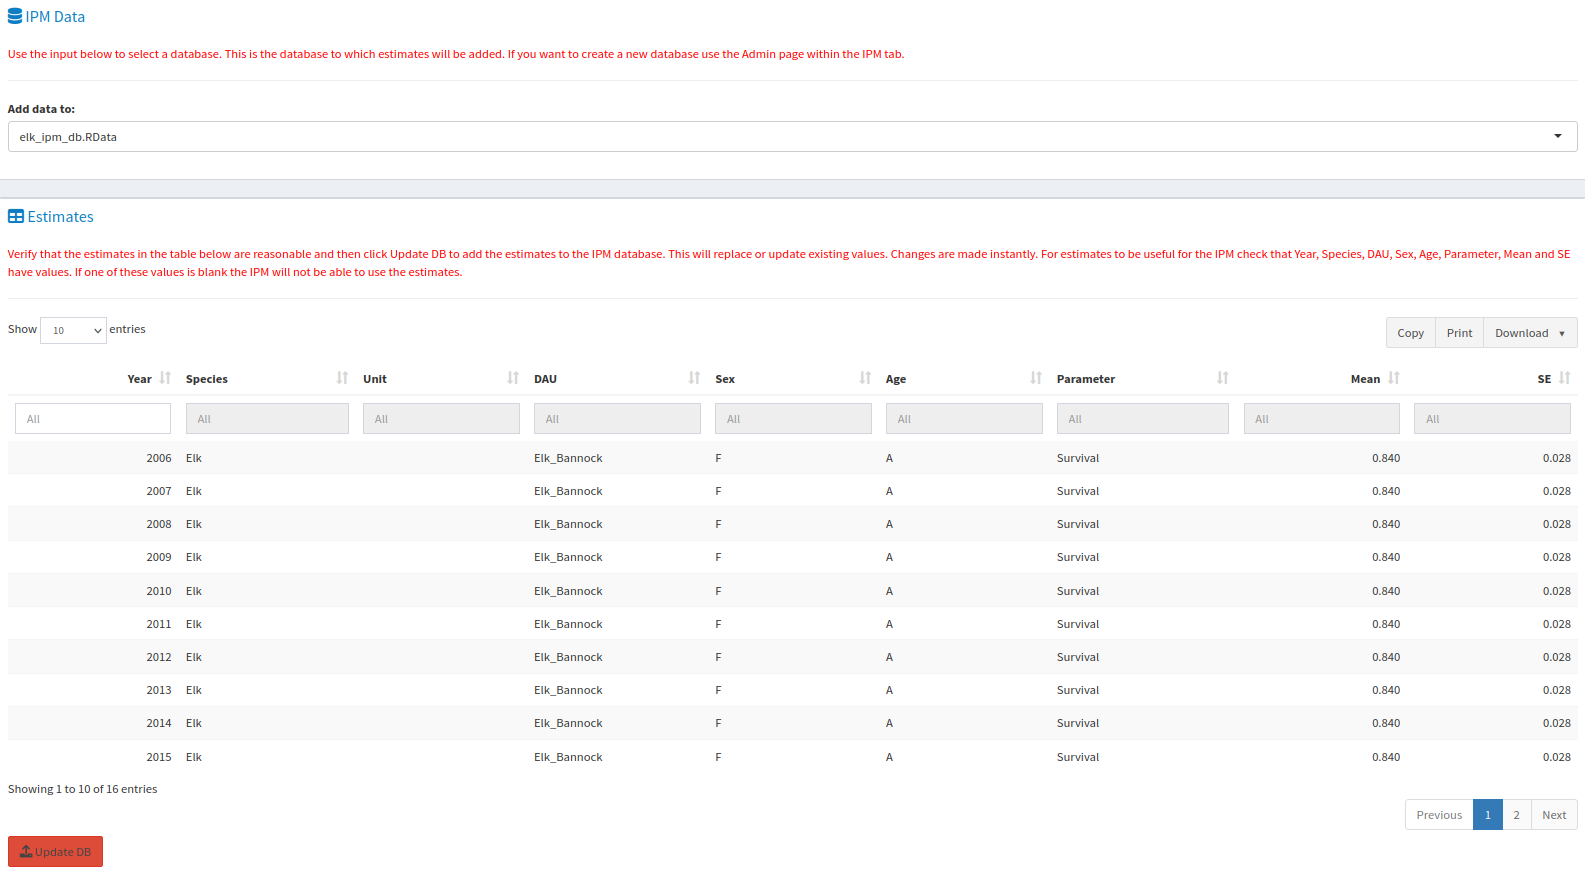
\includegraphics{./www/surv_walk11.png}

\hypertarget{surv-ref}{%
\section{Reference}\label{surv-ref}}

\hypertarget{surv-setup}{%
\subsection{Setup}\label{surv-setup}}

The window on the top left determines how your model is going to be run. The Overview tab is where you select and download the data that you will be modeling for survival by species of animal and DAU that the data was collected in. The only way to preview the data before modeling is to download it, and you will have to redownload if you want to change the species or DAU before you run the model. Data comes from IDFG's Statewide Animal Monitoring Master (SAMM) and data must be modified at the source within SAMM. PopR only loads the data temporarily using an API, and so cannot modify it. The Subset tab lets you decide which sections of your elk or mule deer population will be included in your output, and over what period of time. The default inputs are Sex:All, Age:A.

In the Structure tab, we get to make some decisions about our model. The Default inputs work well for a variety of situations and you should keep them if you plan on putting the results of this model into an IPM dataset. They are: Model Type: Known Fate, Covariates: None, Censor Fate(s): None, Model sexes as: Same, Model time as: Constant, Model space as: Constant. Our options for Model type are known fate and multi state and each has its own strengths and specific use cases (GLOSSARY). You can also select which covariates will be included in your analysis here. Censor fate allows you to remove animals from your analysis who were harvested by hunters. Simply click the Harvest option. Model Sexes can get survival metrics of both males and females separately by setting it to Different. You can model both time and space as both constant and monthly.

The Run tab allows us to control the actual process of running our model. Burnin Length helps us focus our model. When the MCMC model begins running, it checks possible outputs of the model and begins sampling them to determine the probability that they will represent our data. The model uses past sampled points to try and get an idea of where the highest probabilities are, but when the model first begins running it does not have the luxury of these reference points. This sets up the model's first few samples to be more randomly chosen than any part of the process, meaning that the beginning samples are less likely to be on high probability outputs. Burnin Length helps us get around this by deleting the first runs of the MCMC model after it's done running. MCMC iterations is simply a measure of how many different times the model will test the probability of different model outputs. More sampling allows the model to consider more options and therefore can increase the chance that the model will find the outputs with the highest likelihoods, but it also may not be necessary and will make the tool take longer to run. Thinning rate helps us save memory by deleting entries from the model's stored runs. We can think of this as a sort of browser history for the model, showing us how it got its answer. In this case there are literally tens of thousands of steps, so deleting a small (or large) proportion of that history and using what is left still gives us an idea of the model's actions without taking up nearly as much memory. The slider is the percentage of model iterations that will be deleted once the modeling process is complete.

Use the window at the top right of the page to check for data issues. The window to the top right is very useful for troubleshooting. The capture tab displays the ID of an animal that that has bad or no XY data in the capture tab at the bottom of the page. The Mortalities tab displays Mortality data whose XY data needs fixing as well. To get a better idea of which points are causing a problem, points can be clicked on the map to get their IDs as well.

The window at the bottom of the page works as a preview for data that is gathered by the download data button. All of the tables can be downloaded with the corresponding button, but only data that is displayed to be downloaded, so make sure {Show (10) Entries} is changed to ``All'' if you would like to get your entire output in one .csv. All of the tables can be searched using the empty slots at the top of each column. Searching the ID column can be very helpful for finding data that is also displayed in the window that shows entries with damaged xy data. The Raw Data from SAMM, Idaho's database that includes statewide animal monitoring data, is displayed here as well, but as stated above changes to the data will have to be made in SAMM itself.

\hypertarget{surv-admin}{%
\subsection{Admin}\label{surv-admin}}

The Admin tab is a straightforward page used to upload the results of your model to your database of choice. The bottom window can be used to preview the data that you plan to upload, so make sure you are comfortable with your results before you upload them to the public database. Data you upload will be incorporated into everyone else's model runs, so be careful.

\hypertarget{surv-tables}{%
\subsection{Tables}\label{surv-tables}}

Once your model is finished running, you can view the results in the Tables tab. Note that the first ten entries that appear when you open this page are only a small fraction of the total. Use the page list on the bottom right to see more pages of data or use the dropdown menu on the top left to make more entries appear on each page.

\hypertarget{surv-indiv}{%
\subsection{Individuals}\label{surv-indiv}}

If the window in the setup tab shows that there may be problems with XY data in capture and mortalities, this is the place to go. After selecting your individual of interest at the top of the page, the bottom two windows show all data available. Raw data from SAMM, Idaho's statewide database, is on the left and data formatted by speedgoat for our model is on the right. There are many columns, so make sure to scroll horizontally to make sure you see them all. The empty text box at the top of each column allows you to do a search.

\hypertarget{de}{%
\chapter{Data Entry}\label{de}}

This tool handles/organizes the information that makes all of the other tools work. More specifically, the data entry tool allows you to design sightability and composition surveys for a DAU and then enter/upload the results to the speedgoat database. Remember that the surveys you create and edit are the same ones that everyone on your team has access to, so any edit you make will change the data that EVERYONE is using for analysis.

\hypertarget{de-walk}{%
\section{Walkthrough}\label{de-walk}}

The data entry tool can be broken into two sections: creating a survey and then filling it with data.

\hypertarget{de-create}{%
\subsection{Creating a Survey}\label{de-create}}

You can use the data entry tab to design aerial surveys and then populate them with data, which can then be used to inform our survival, sightability, and IPM tools.

To begin designing a survey click the Survey Design tab.

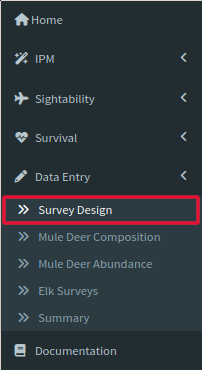
\includegraphics{./www/de_walk1.png}

When you click the page, a popup window labeled Survey Design Setup should appear, prompting you for your survey species, DAU, survey type, and survey year.

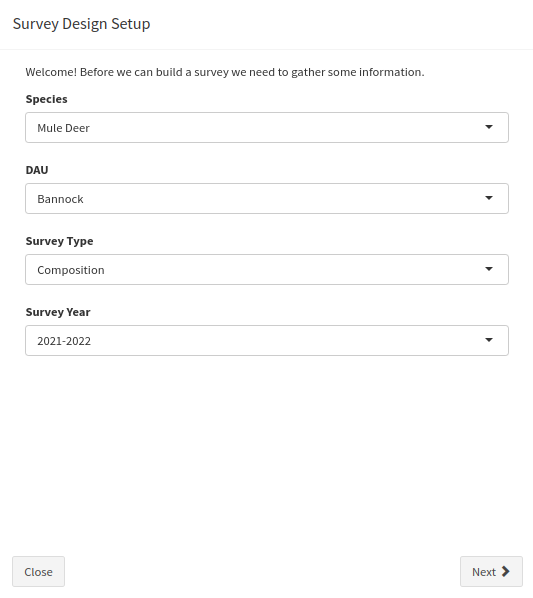
\includegraphics{./www/de_walk2.png}

If this window does not pop up click the gear icon on the bottom left of the page and select {Setup Wizard}.

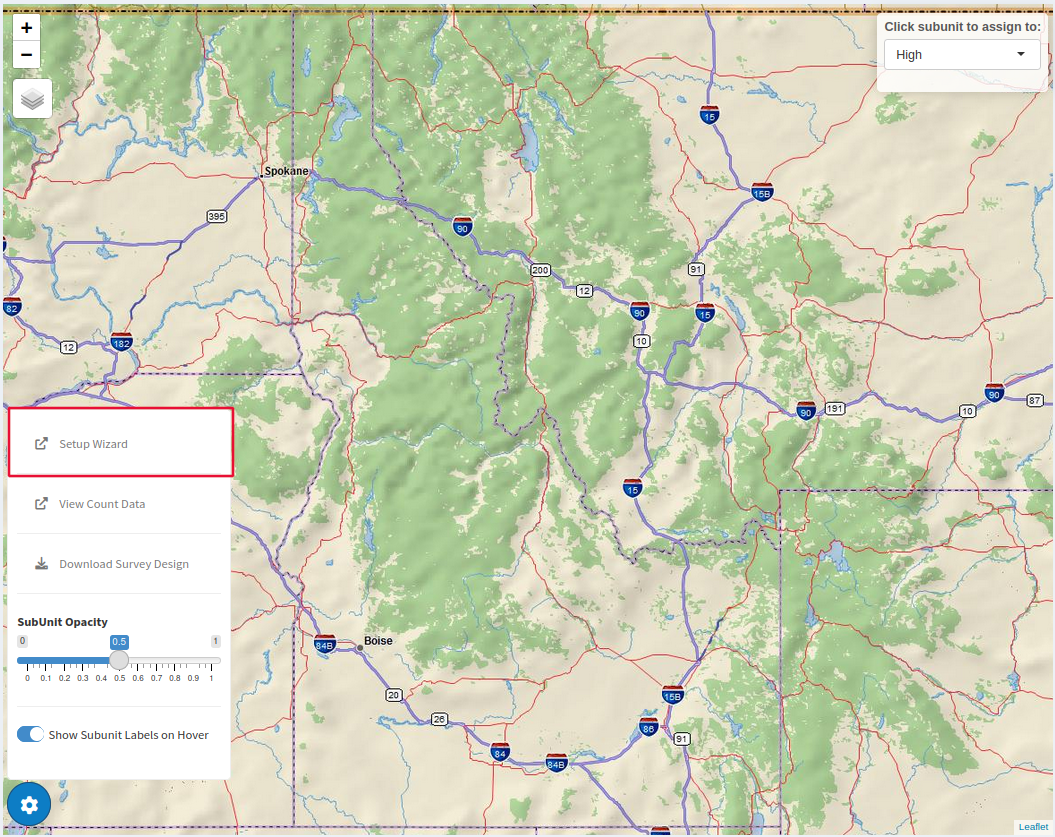
\includegraphics{./www/de_walk3.png}

Once you have made your choices, a second window will appear asking you whether you would like to import strata from a past survey or start from scratch.

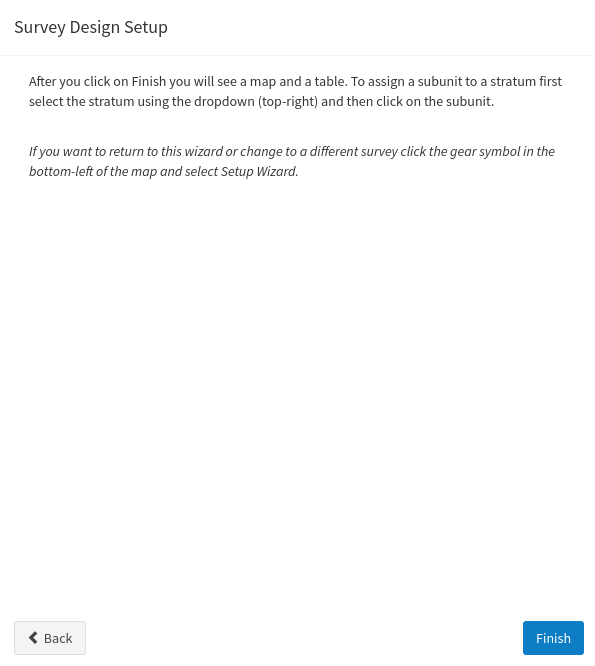
\includegraphics{./www/de_walk4.png}

Either way, clicking {Finish} on this second window will close the popup and leave you with a map and a table. The map and the table both act as options to assign subunits to different strata, which is the next step in the process.

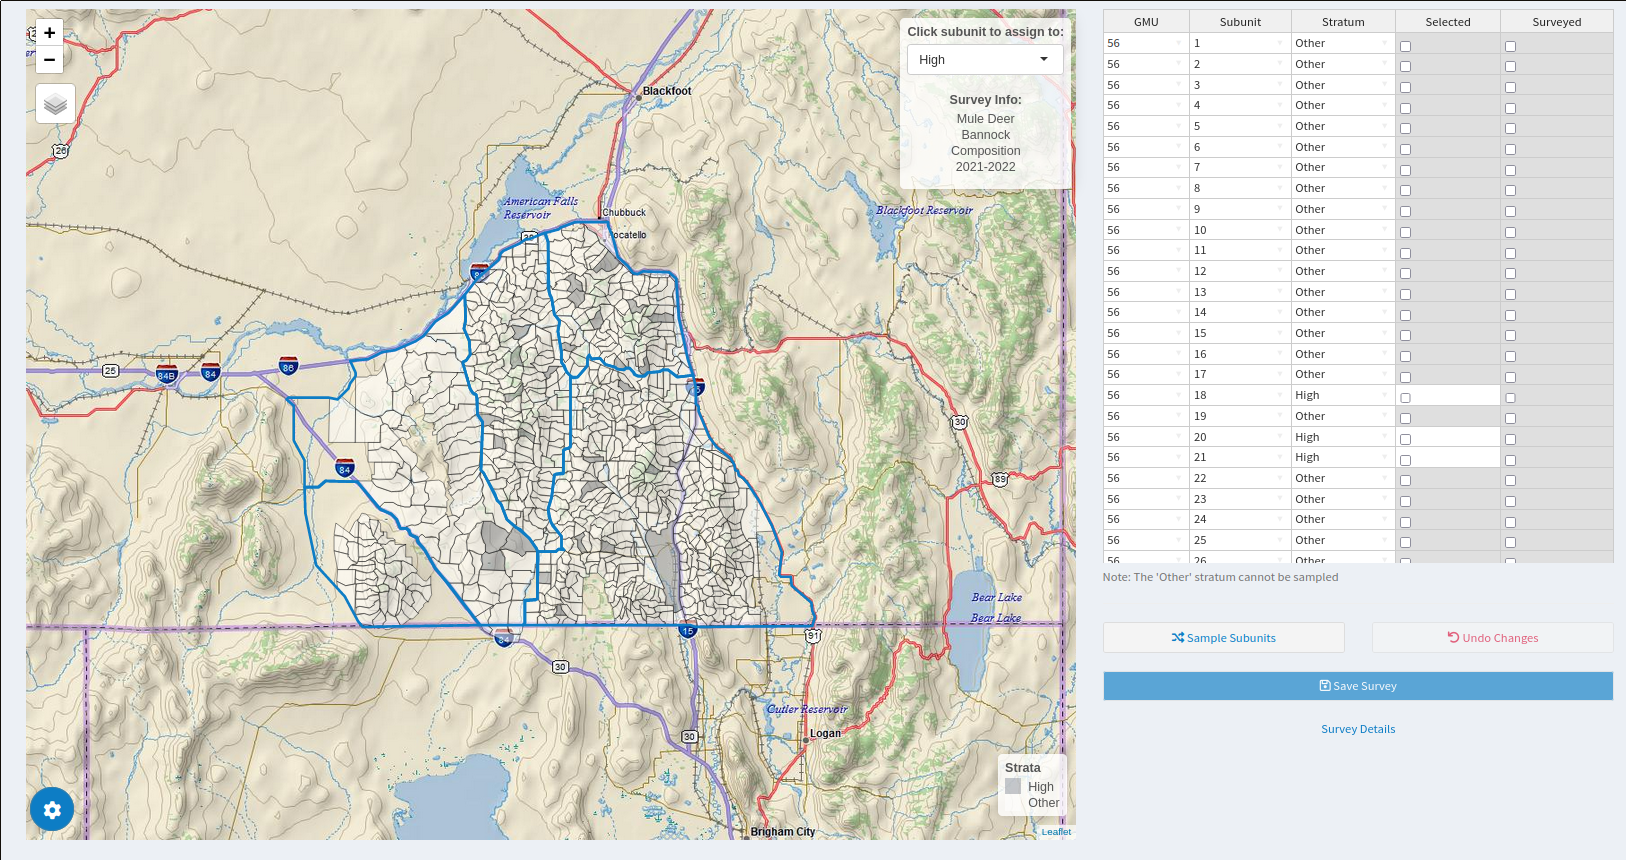
\includegraphics{./www/de_walk5.png}

To use the map, choose which strata you would like to assign to the subunits with the small window labeled Click Subunit to Assign to: and then once your strata is selected, all subunits you click on the map will be assigned to that strata.

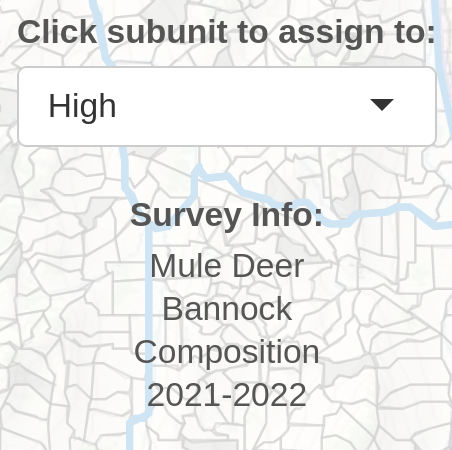
\includegraphics{./www/de_walk6.png}

You can also assign subunits to different strata by using the table to manually change the Stratum column from Other to whichever is appropriate for your experiment. Note that any subunit left in the Other strata will not be sampled.

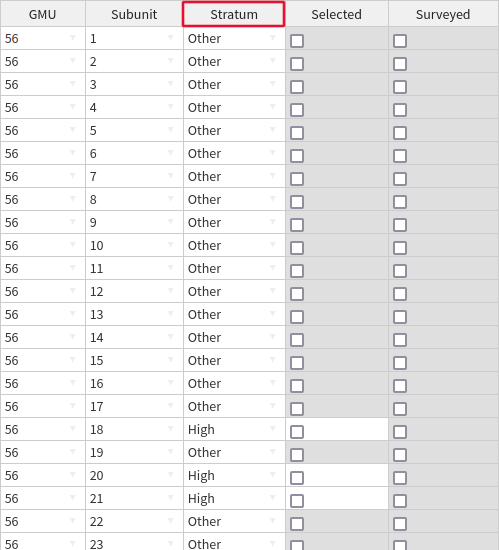
\includegraphics{./www/de_walk7.png}

After you have selected the subunits you plan to fly, click {Sample Subunits} to decide the time to fly each subunit, the proportion of the High strata that will be sampled, and whether you will sample randomly or using GRTS.

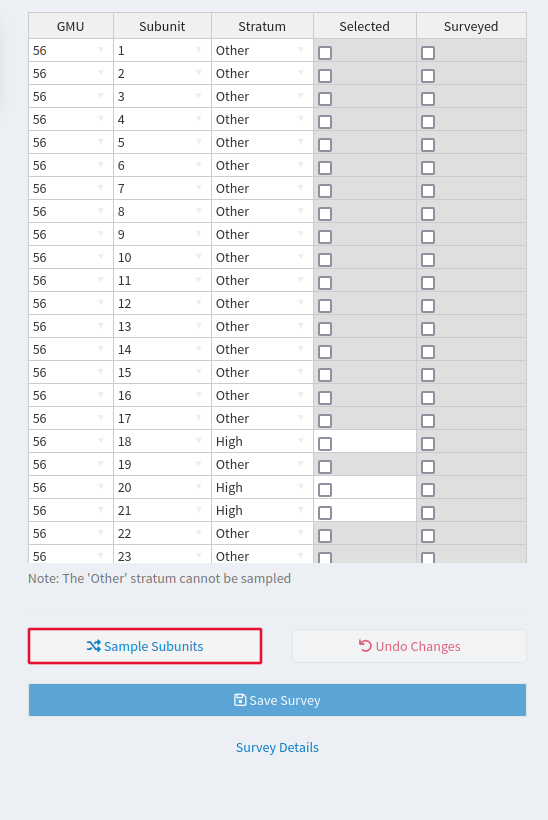
\includegraphics{./www/de_walk8.png}

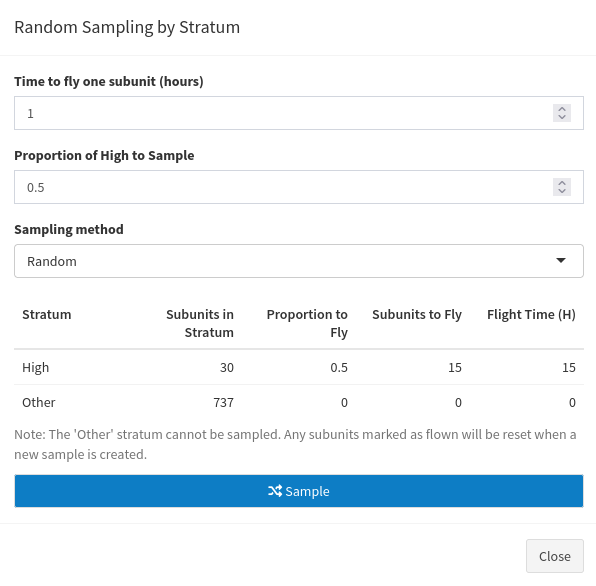
\includegraphics{./www/de_walk9.png}

When you are satisfied with the survey you have designed, Click {Save Survey} to save your edits.

When your survey is actually flown, return to the survey and check the Surveyed box to signal which subunits (of the units selected to be part of the survey earlier) have actually been flown. Click {Save Survey} to save your edits.

\hypertarget{de-popul}{%
\subsection{Populating the Survey}\label{de-popul}}

Now that you have generated at least one survey, it is time to learn about the Mule Deer Composition, Mule Deer Abundance, and Elk Surveys tabs under the Data Entry dropdown, which are all used to populate surveys created in the Survey Design tab.

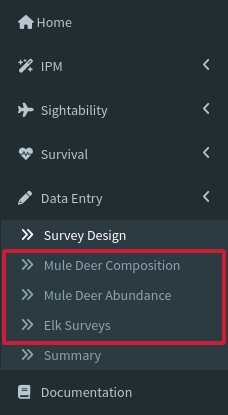
\includegraphics{./www/de_walk10.png}

It is important to understand that data added here will modify the surveys for EVERYONE, so make sure you are comfortable with this information being used for analysis if you add it here.

All three of these tools use the same framework for data entry. To make sure you're adding info to the right survey you can either enter the relevant info in the upper window or use {click here} the top of the page, which allows you to hunt for your survey manually.

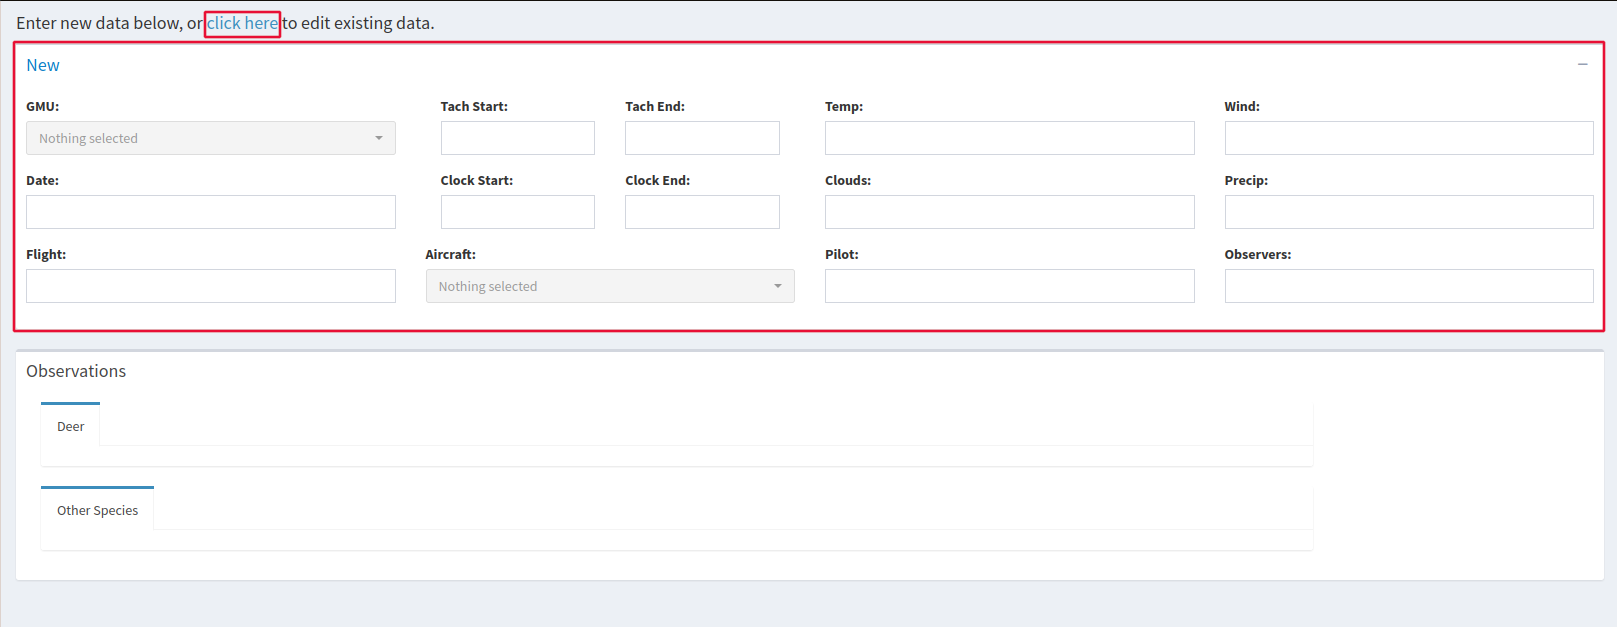
\includegraphics{./www/de_walk11.png}

When you have selected your survey, you can add data manually one entry at a time, which is done by clicking any of the dropdown arrows in the cells of the Observations table. If you already have a spreadsheet prepared, you can also copy and paste that information right into the table.

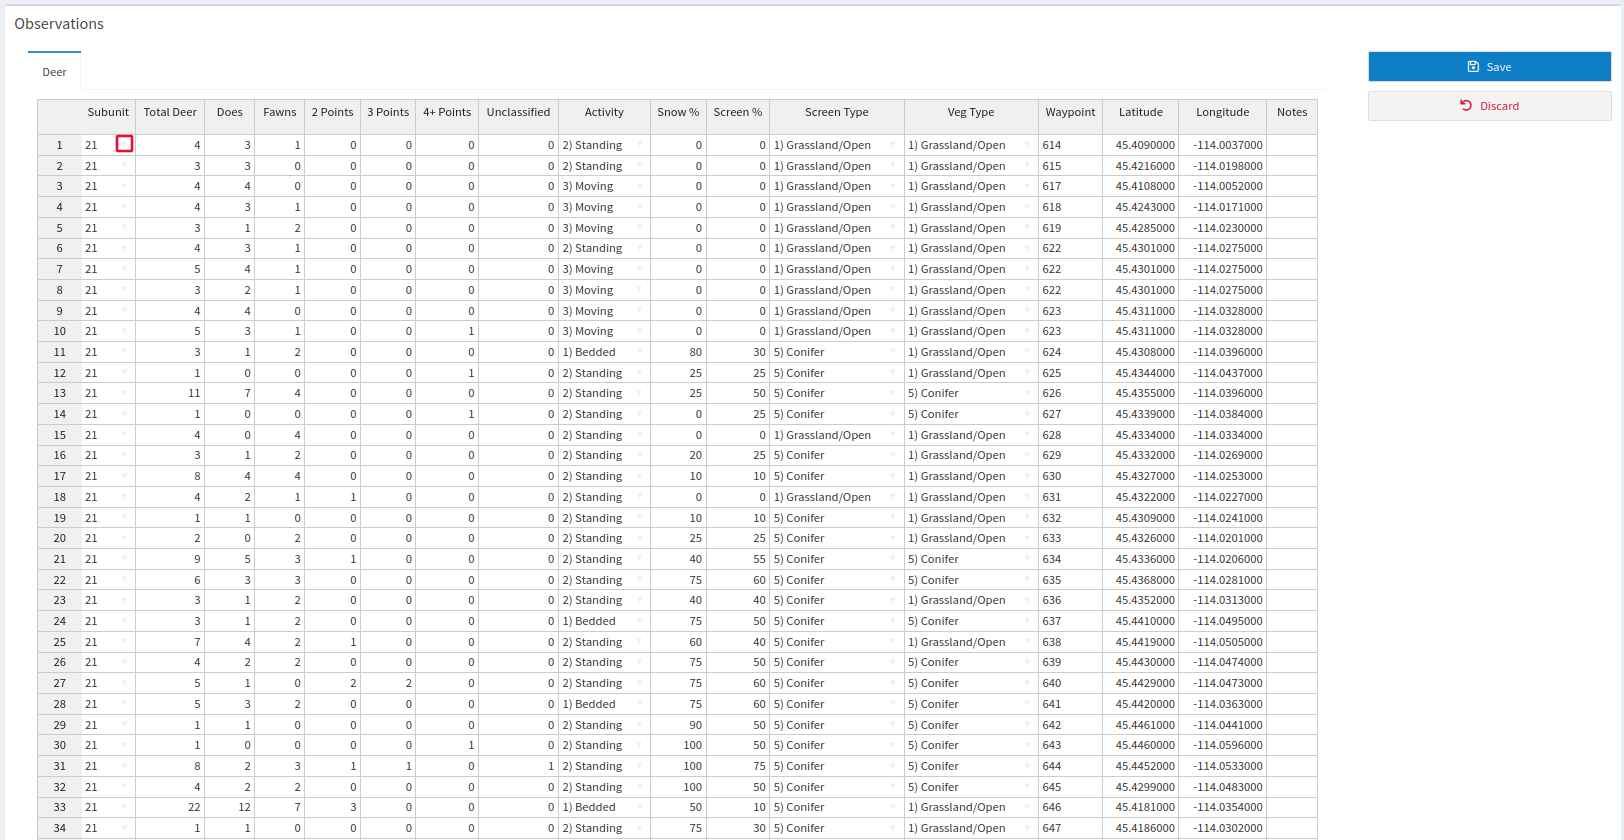
\includegraphics{./www/de_walk12.png}

While you make these edits, the area that normally displays {Add GPS Data} and {Totals} changes to {Save} and {Discard}. Either accept your changes and save them to your database with {Save} or revert any changes with {Discard} and the original options will reappear.

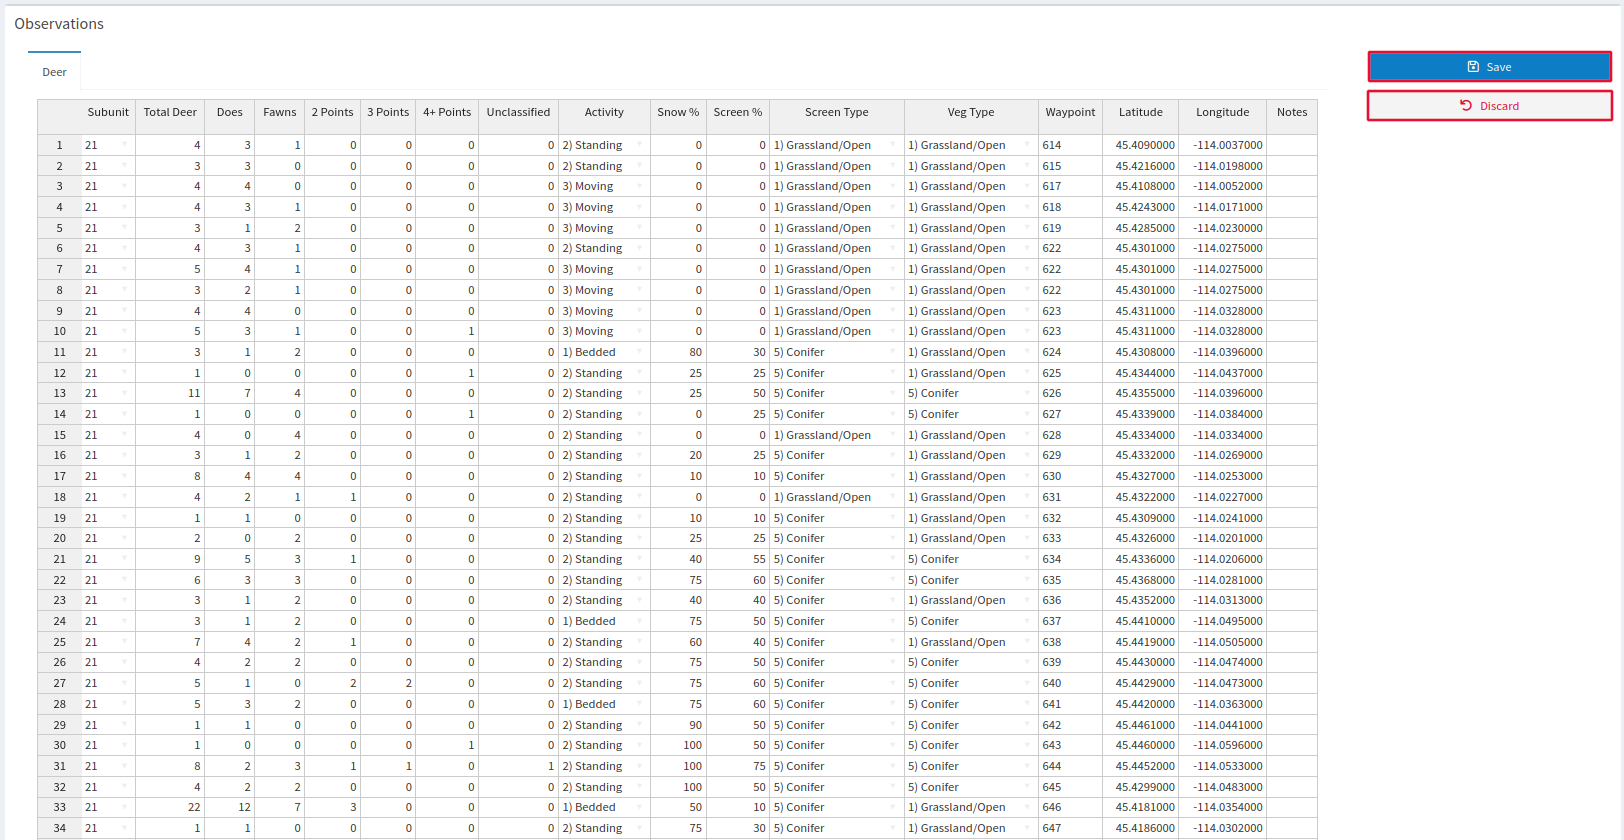
\includegraphics{./www/de_walk13.png}

You can add latitude and longitude information to the database with {Add GPS Data} on the right side of the page, which will be visible as long as you do not have any unsaved edits to your Observations table. Follow the instructions of the popup window that appears for final import instructions.

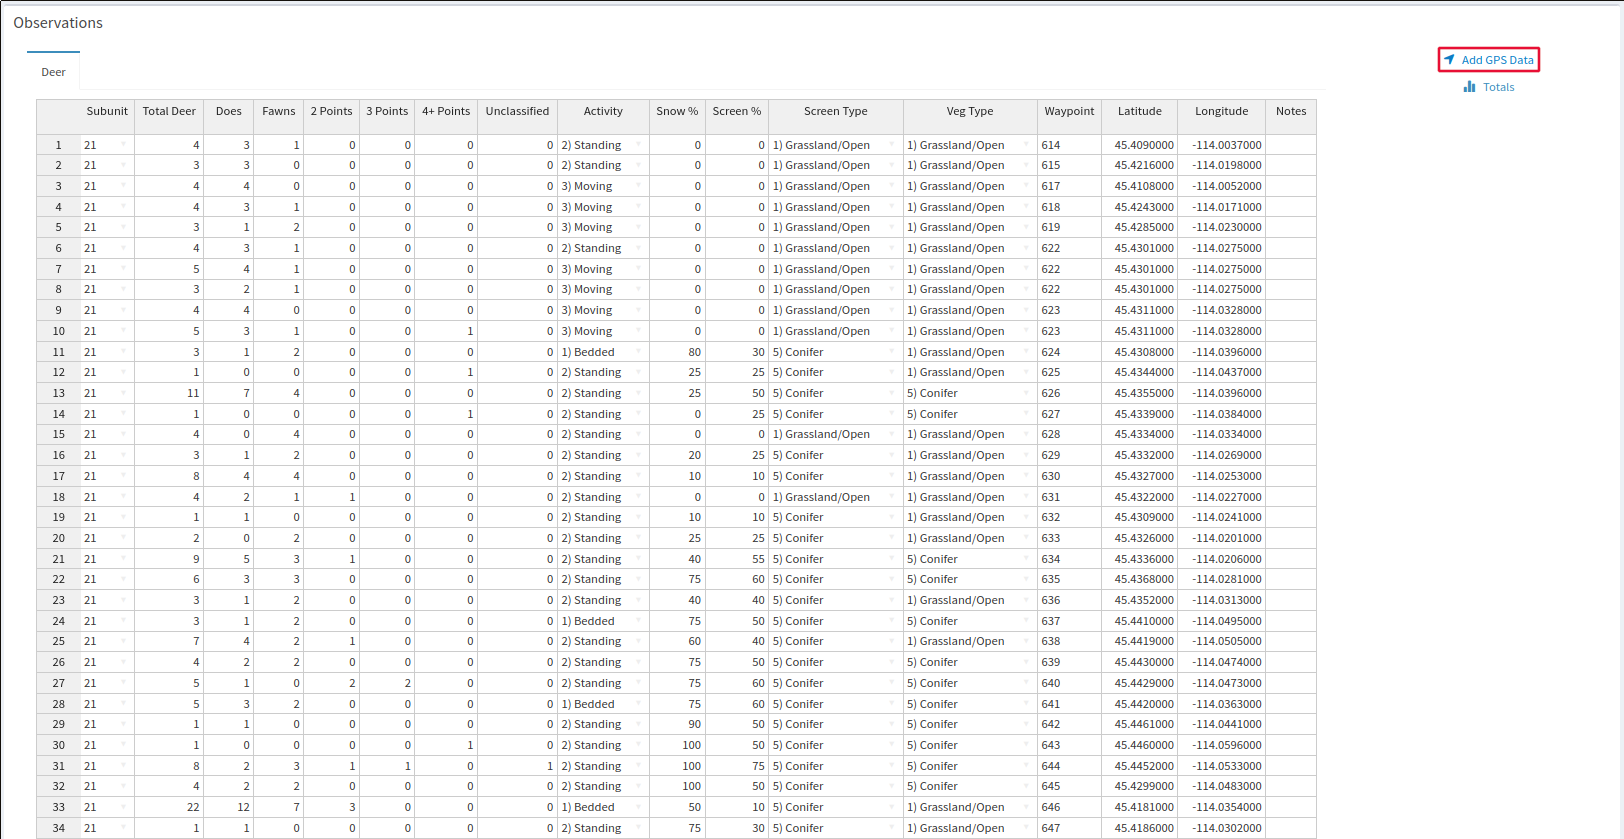
\includegraphics{./www/de_walk14.png}

When you are finished, make sure you click {Save} to make your changes permanent. {Attached Files} allows you to add files like maps and raw data for future reference and redundancy.

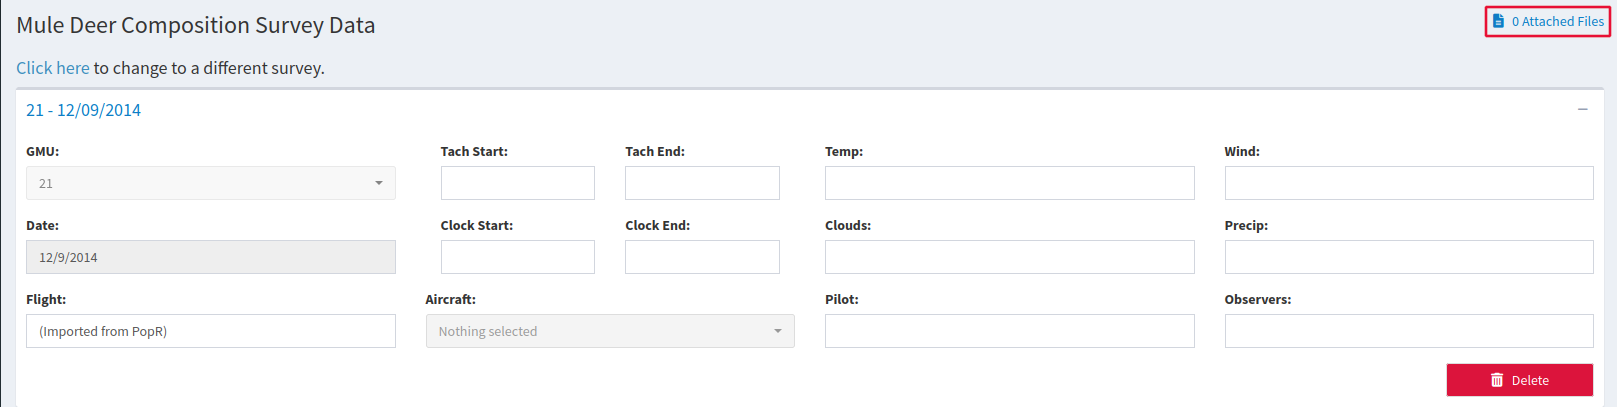
\includegraphics{./www/de_walk15.png}

\hypertarget{de-ref}{%
\section{Reference}\label{de-ref}}

\hypertarget{de-surdes}{%
\subsection{Survey Design}\label{de-surdes}}

Though someone with intimate knowledge of an area can bring a survey team to an area where there are a relatively high abundance of deer, surveys that return very low abundance are important as well in order to fully inform the model. The model assumes density to be constant, so if you only fly subunits where you know there are a lot of animals, that amount of animals will be extrapolated to your entire DAU and can lead to overestimation, since your DAU is now represented by only its busiest areas. If you want to track how many subunits are going to be included in your analysis, click {Survey Details} below the subunit selector table. This menu will remind you of your model settings while showing how many subunits have been selected for survey and how many have actually been surveyed. Make sure you stick to your predetermined selections if you want the model to return relevant information, since it is expecting data from these areas and these and these areas only. If the survey design menu does not pop up when you open the tool, then click the gear button on the bottom left of the page and select Setup Wizard from the options in the popup menu.

\hypertarget{de-mdcomp}{%
\subsection{Mule Deer Composition}\label{de-mdcomp}}

This software can only use data from aerial surveys. There is an option to select the aircraft that was flown for the survey which is considered for elk sightability surveys but NOT mule deer surveys, so it's best to just leave that box as ``Nothing Selected''. You can either begin entering survey data manually in the window labelled New, which will begin adding your data to a new survey, or you can edit surveys that you have already created with the link above the table labeled ``click here''. The Attached Files button Allows you to add files that you would like to be kept with your observations such as a reference map.

The Observations window allows you to view and alter your data. The Add GPS Data button on the right side of the window allows you to easily import latitude and longitude from .csv files, and the Totals button brings up a window summarizing your data.

\hypertarget{de-mdabun}{%
\subsection{Mule deer Abundance}\label{de-mdabun}}

This software can only use data from aerial surveys. There is an option to select the aircraft that was flown for the survey which is considered for elk sightability surveys but NOT mule deer surveys, so it's best to just leave that box as ``Nothing Selected''. You can either begin entering survey data manually in the window labelled New, which will begin adding your data to a new survey, or you can edit surveys that you have already created with the link above the table labeled ``click here''. The Attached Files button Allows you to add files that you would like to be kept with your observations such as a reference map.

The Observations window allows you to view and alter your data. The Add GPS Data button on the right side of the window allows you to easily import latitude and longitude from .csv files, and the Totals button brings up a window summarizing your data.

\hypertarget{de-esurv}{%
\subsection{Elk Surveys}\label{de-esurv}}

Like the mule deer survey tools, this software can only use data from aerial surveys. Elk sightability models are different than the mule deer ones since they incorporate the make of the survey plane in the model. Either enter data from your survey directly to begin adding data to a new survey or by clicking the ``Click Here'' under the page header. The Attached Files button Allows you to add files that you would like to be kept with your observations such as a reference map.

The Observations window allows you to view and alter your data. The Add GPS Data button on the right side of the window allows you to easily import latitude and longitude from .csv files, and the Totals button brings up a window summarizing your data.

\hypertarget{de-summ}{%
\subsection{Summary}\label{de-summ}}

Be aware that the surveys displayed in the table when you first open the tool are not all of the data available, use the page navigation at the bottom right of the window to see more. If you are looking for a particular survey or location, the blank boxes at the top of every column can be used to search all entries. Just type something in the box and it will automatically find entries in the column that match what you type. This section is great for reviewing/checking raw data since you can download any of the survey data as a .csv.

\hypertarget{gl}{%
\chapter{Glossary}\label{gl}}

\textbf{Beta:} The strength of each variable in the model itself. Categorical variables are represented by a range of binned values, but for the model to create an output it must be converted to a numerical value that modifies the default value. For example, the VegClass covariate changes how easy it is to see an animal. VegClasses differ in the amount that they can obscure vision, but you will notice the classes that obscure visions the most have a negative beta value, which tells us that they have a negative impact on our probability to see an animal.

\textbf{Composition survey:} A sightability survey which focuses on sex ratios

\textbf{DAU:} Data Analysis Units separate Idaho into distinct management areas for each species. Each one has a specific name and is further divided into subunits, which allow even more specificity.

\textbf{Model value:} The numerical value that the model assigns to different covariates. In the User Interface, different covariates have helpful labels like ``Snow Cover'', but in actual programming language this would make code unnecessarily long and complicated, so the computer stores them as simple numerical values instead.

\textbf{Sightability-Abundance Survey:} A sightability survey which focuses on abundance

\textbf{Stratum:} Stratum are used to organize habitat subunits by how well they would work as habitat for the animal being surveyed. The ``high'' strata group represents subunits that contain the best habitat, ``low'' is the group that has the worst habitats, and ``medium'' falls in between. Subunits are determined by previous observations from biologists and snow cover.

\end{document}
